%-------------------------------------------------------------------------------
%	CAPITOLO 29
%-------------------------------------------------------------------------------
%
\chapter{I maestri di lingua - Araldo il Capolega B...}
\index[Personaggi]{Lanconelli Araldo}Araldo\footnote{\textbf{Araldo Lanconelli},  tutto ciò che so di lui è che sua figlia si chiamava Angelina e che questa fu presente al matrimonio di \index[Personaggi]{Marini Marino}Marino Marini. Tuttavia, Mingazzi ci suggerisce che Araldo coprì la carica di assessore.}, seduto, calvo, con la coppole sulla cervice, ben nutrito, baffi, spioventi, alla moda, era un bell'uomo. Dritto non ci stava perché era zoppo... e così nelle concioni\footnote{Discorso solenne fatto in pubblico, arringa (nell’uso moderno ha spesso valore ironico o spregiativo)} dei repubblicani, si vestiva di nero e si metteva in evidenza nel palco accanto a \index[Personaggi]{Mirabelli Roberto (onorevole)}Mirabelli\footnote{\textbf{Roberto Mirabelli}, onorevole, di origine calabrese, più volte deputato di Ravenna per il PRI} o \index[Personaggi]{Mazzolani Ulderico (onorevole)}Mazzolani\footnote{\textbf{Ulderico Mazzolani}, onorevole repubblicano}, essendo un bel pezzo... decorativo.\\
\indent Con le sue idee repubblicane non transigeva, era attaccato alla carica e fu anche assessore.\\
\indent Una sera, durante l'assessorato, si recò a casa, come d'abitudine all'ora di cena, del \index[Personaggi]{Meruzzi dott. Cassiano}Dr. Meruzzi\footnote{Dr. \textbf{Cassiano Meruzzi}, medico condotto di Alfonsine, cugino di Cassiano Bagnara, figlio di Giovanni, proprietario della casa di Vincenzo Monti.}. Poveretto non stava più nella pelle, rideva, si contorceva, faceva delle smorfie.\\
\indent Allora cominciò questo dialogo:\\
\indent Dr. Meruzzi\index[Personaggi]{Meruzzi dott. Cassiano}: <<Insomma, sei troppo contento... hai qualche cosa, dillo.>>\\
\indent \index[Personaggi]{Lanconelli Araldo}Araldo: <<Ecco. Noi repubblicani, a fasèn un oratorio a què drì a la mura d'Terulin\footnote{<<Noi repubblicani facciamo un oratorio qua dietro le mura di Terulin>> - (ndr) non ho trovato corrispondenze con `Terulin'}>>.\\
\indent Donne di casa: <<Oh! Bene così andiamo a pregare... è vicino.>>\\
\indent \index[Personaggi]{Lanconelli Araldo}Araldo si rabbuia e tace.\\ 
\indent \index[Personaggi]{Meruzzi dott. Cassiano}Dr. Meruzzi: <<Voi repubblicani, mangia preti, non ci sarebbe altro... che faceste proprio una chiesa.>>
\indent \index[Personaggi]{Lanconelli Araldo}Araldo in fretta: <<Ma che cisa, a fasèn un pisadur!\footnote{<<Ma che chiesa, facciamo un pisciatoio!>>}>>.\\
\indent \index[Personaggi]{Meruzzi dott. Cassiano}Meruzzi e donne risposero con una risata e poi <<Puh!>>\\
\indent \index[Personaggi]{Meruzzi dott. Cassiano}Meruzzi: <<Alora té da dì un orinatoio...\footnote{<<Allora devi dire orinatoio>>}>>\\
\indent \index[Personaggi]{Lanconelli Araldo}Araldo: <<L'è l'istes, l'è question d'paròl\footnote{<<È lo stesso è questione di parole>>}>>\\
\indent Era anche assessore alla pubblica istruzione certamente se ne intendeva molto e poteva dire anche altro.

Un altro giorno il nostro \index[Personaggi]{Lanconelli Araldo}Araldo, raccontava: <<L'ha scrèt a cà \index[Personaggi]{Forlivesi Sebastiano `Nisò d'Furlivési' (commerciante)}Nisò d'Furlivési\footnote{\textbf{Forlivesi Sebastiano}, nato nel 1830 e morto nel 1905, è il primo dei quattro alfonsinesi che in un modo o nell'altro furono coinvolti nelle varie imprese garibaldine. Partecipò fin dall'inizio alla difesa della Repubblica Romana (1849). Con l'unità d'Italia ebbe a ricompensa della sua attività garibaldina il permesso di aprire una bottega. Quella bottega, passando di figlio in figlio, è ancora oggi attiva in Corso Garibaldi ed è sempre stata chiamata "Butega dla Formazala".} cl'à sintì \index[Personaggi]{De Maria Ugo (professore)}Ugo d'De Maria\footnote{\textbf{Ugo De Maria}, libero docente dell'Università di Parlemo. Fu allievo del Carducci.} in piaza a Palermo, che siringava la folla, contra a Nasi\footnote{<<Ha scritto a casa Nisò d'Forlivesi che ha sentito Ugo De Maria in piazza a Palermo che siringava (per arringava) la folla>>}>> (era il tempo dello scandalo Nasi\footnote{Il Ministro della Pubblica Istruzione, Nunzio Nasi venne accusato di gravi irregolarità nel suo operato. Si parla di corruzione, sussidi ingiustificati, firme sospette, favoritismi, spese personali pagate con i soldi pubblici.})\\
\indent Speriamo che il buon Dio tenga lontano ai palermitani il mal d'urina! Ce ne sarebbero troppe, ma finiamo con l'ultima.\\

\vspace{0.5cm}
\centerline{\rule{1.5cm}{0.4pt}}
\vspace{0.5cm}

Un giorno, al nostro Araldo viene consegnata la scheda per il censimento della popolazione. Da letterato si mette subito all'opera.\\

\textcal \Huge
Araldo L\:.\:.\:.\: fu \:.\:.\:.\:\\
\normalfont \normalsize
di professione:
\textcal \Huge Agente Urale
\normalfont \normalsize (per `rurale')\\
di religione: 
\textcal \Huge Ateo

\normalfont \normalsize

\indent Speriamo bene che il nostro protagonista non vada alla storia... e che la scheda di suo pugno non vada in bella mostra... in vetrina.\\

\vspace{0.5cm}
\centerline{\rule{1.5cm}{0.4pt}}
\vspace{0.5cm}


Nel momento rosso i socialisti avevano caricato un buon uomo di molte frasi, capite come poteva e secondo lui solo\footnote{Interpretate a modo suo}.\\
\indent Necessitava una concione\footnote{Discorso solenne in pubblico}.\\
\indent Il nostro uomo, rosso, forte, gesticolante cominciava.\\
\indent <<Soci, amici, compagni, sucilèsta, d'la sucietè, d'la fratelênza, d'la adunênza, d'la cumbrècula, d'la sozia di cuntadèn.\footnote{<<Soci, amici, compagni, socialisti, della società, della fratellanza, dell'adunanza, della combriccola, della socia dei contadini>>}>> Punto e basta il repertorio era esaurito con un <<Evviva noi!>>\\
\indent Per sentire questo discorso migravano molte staffette, parecchi giorni prima; ed il giorno  dell'adunanza i contadini irreggimentati.\footnote{Si muovevano in molti per ascoltare ed il giorno dell'adunanza era tutti inquadrati e pronti all'ascolto} \\
\indent Si vede che mancavano persone a conteggiare quante suole delle scarpe... costava la concione.

 \begin{figure}[htb]
    \centering
    %\vspace{-0.7cm}
    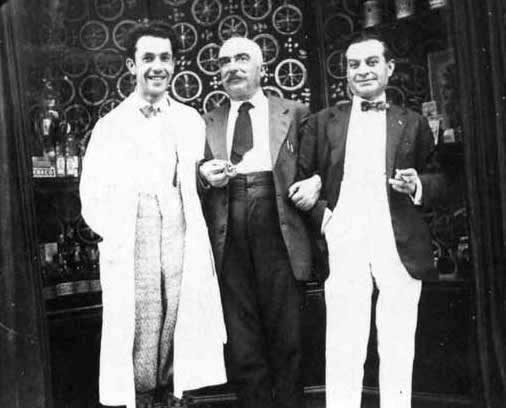
\includegraphics[width=\textwidth]{meruzzi}
    \caption[Farmacisti della farmacia comunale in via Mazzini]{I farmacisti della farmacia comunale \index[Luoghi]{Farmacia Comunale} di via Mazzini appartenuta ad \index[Personaggi]{Boari Attilio (farmacista)}Attilio Boari. Partendo da sinistra: Dr.\:\index[Personaggi]{Stella dott. Domenico}Domenico Stella, \textbf{Dr.\:Cassiano Meruzzi}\index[Personaggi]{Meruzzi dott. Cassiano}, Nando \index[Personaggi]{Isani Nando}Isani.\label{fig:meruzzi}}
    %\vspace{-0.3cm}
\end{figure}










































%
